\subsection{An\'alisis de Tiempo de C\'omputo}
\label{subsec:exp4}
\begin{LaTeXdescription}
    \item[Objetivo] Analizar la complejidad temporal del m\'etodo.\\

    \item[Hip\'otesis] Proponemos que el tiempo de c\'omputo por iteraci\'on
        para una instancia y $\epsilon$ fijos ser\'a siempre el mismo para todo
        $\alpha$. Tambi\'en proponemos que el tiempo de c\'omputo por interación
        para $\epsilon$ fijo ser\'a el mismo para \textbf{toda instancia} (sin
        importar tama\~no, cantidad de ejes, etc).\\

    \item[Proposici\'on] De los experimentos previo hemos llegado a la
        conclusi\'on de que a mayor $\alpha$, mayor cantidad de iteraciones
        ser\'an necesarias para converger, lo cual implica inmediatamente un
        mayor tiempo de c\'omputo requerido. La pregunta ideal a responder
        ser\'ia ''cu\'anto tiempo'', pero tambi\'en concluimos previamente que
        la cantidad de iteraciones es dependiente (entre otros factores) de la
        instancia de entrada. Con lo cual, responder a esta pregunta en el
        contexto de este trabajo es imposible sin una cota te\'orica para la
        cantidad de iteraciones (que ni siquiera sabemos si existe). En cambio,
        lo que s\'i podemos analizar es si el tiempo de c\'omputo \textbf{por
        iteraci\'on} es el mismo para toda instancia, sin importar el
        $\epsilon$\footnote{M\'as all\'a de para nuestros experimentos lo
        estemos dejando fijo.} o $\alpha$. Analizamos entonces si el tiempo por
        iteraci\'on var\'ia seg\'un la densidad de la instancia inicial, y a su
        vez si varía para distintos valores de $\alpha$.\\

    \item[M\'etodo de Experimentaci\'on] Tomamos 3 instancias de tama\~no
        mediano-grande, con una diferencia relativa de densidad entre ellas
        significativa. Particularmente, tomamos las mismas del experimento
        anterior. Luego resolvemos cada instancia con PageRank 10 veces para
        $\alpha=0.0$; $0.1$; $0.2$; $\dots$; $0.9$\footnote{Totalizando un total
        de 300 corridas del m\'etodo (10 corridas para 10 valores de $\alpha$
        para 3 instancias distintas).}. Tomamos entonces para cada instancia y
        $\alpha$ fijos, el promedio de los tiempos de c\'omputo. Por \'ultimo,
        calculamos el tiempo de c\'omputo por iteraci\'on dividiendo este
        promedio por la cantidad de iteraciones totales que necesit\'o el
        m\'etodo para converger.\\

    \item[Resultados, an\'alisis y discusi\'on]
\end{LaTeXdescription}

\par Consideramos 2 enfoques para extraer conclusiones, el primero analiza el
tiempo consumido por iteración por el método de la potencia para diferentes
valores de $\alpha$ y el segundo se centra en el tiempo por iteraci\'on respecto
de la densidad de la instancia/grafo de entrada\footnote{Al referirnos a
\emph{densidad} de un grafo, nos referimos a la cantidad de ejes que tiene. A
mayor cantidad de ejes, m\'as denso es.}.

\begin{figure}[H]
    \centering
    \caption{An\'alisis de Tiempo de C\'omputo} %en funci\'on de $\alpha$}
    \subfloat[][Tiempo por Iteraci\'on en funci\'on de $\alpha$.]{
        \label{subfig:exp4_tiempo_iteracion}
        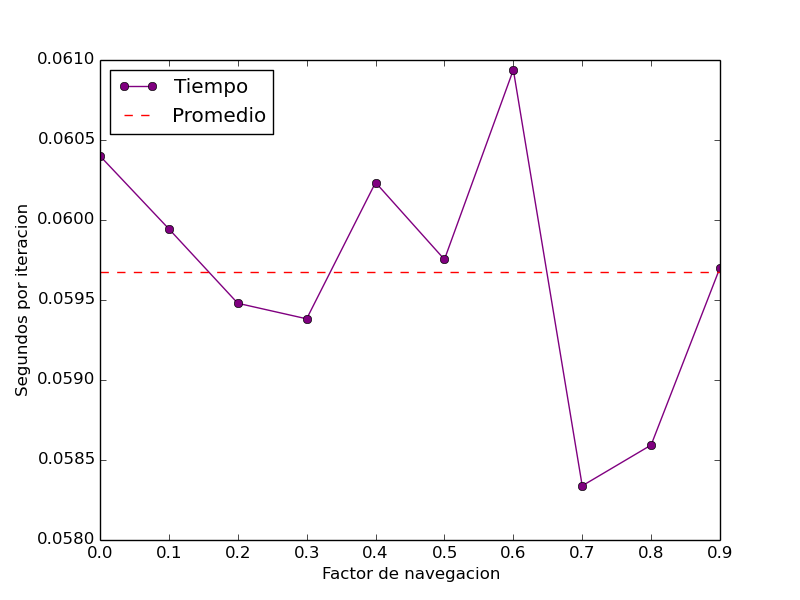
\includegraphics[width=.55\textwidth]{exp4_tiempo_por_iteracion_notredame.png}
    }
    %\begin{figure}[H]
    %    \centering
        \subfloat[][Tiempo por Iteraci\'on promedio vs Densidad del Grafo]{
            \label{subfig:exp4_den}
            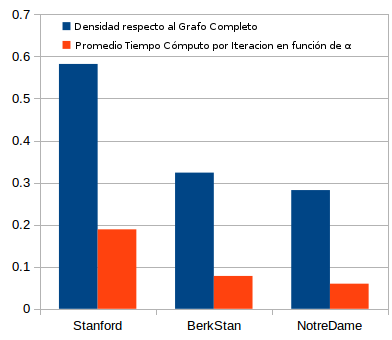
\includegraphics[width=.45\textwidth]{exp4_tiempo_vs_densidad.png}
        }
        %\caption{An\'alisis de Tiempo de C\'omputo en funci\'on de la densidad del Grafo}
    %\end{figure}
    %\subfloat[][Tiempo por Iteraci\'on en funci\'on de $\alpha$. Escala logarítmica]{
    %    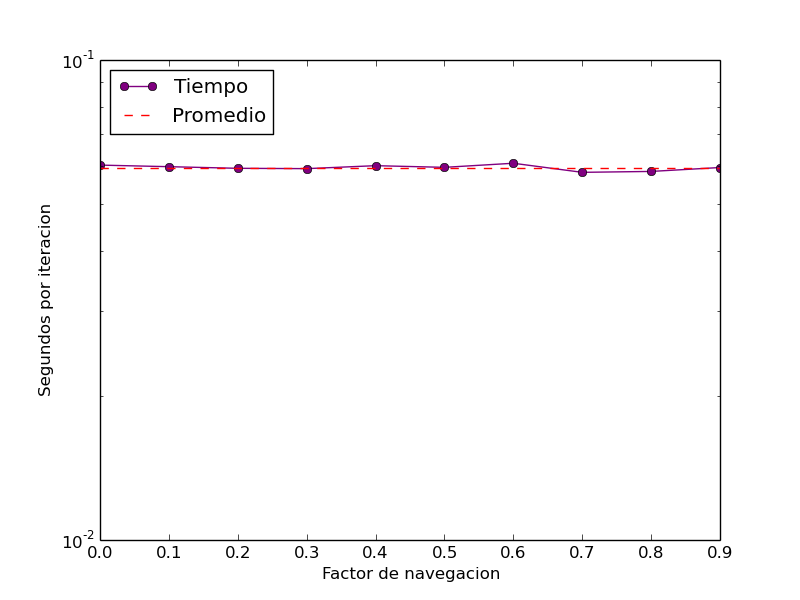
\includegraphics[width=.45\textwidth]{exp4_tiempo_por_iteracion_notredame_log.png}
    %    \label{subfig:exp4_tiempo_iteracion_log}
    %}
\end{figure}

\par Para el primer enfoque, observemos los resultados obtenidos en la figura
\ref{subfig:exp4_tiempo_iteracion}. En el mismo observamos dos curvas. La
primera, \emph{Tiempo}, que representa el tiempo por iteraci\'on promedio para
cada $\alpha$ (calculado como el tiempo promedio hasta converger de las 10
ejecuciones para un $\alpha$ fijo, dividido por la cantidad de iteraciones que
necesit\'o); y la segunda \emph{Promedio} que no es otra cosa que el promedio de
los tiempos por iteraci\'on calculados para la curva \emph{Tiempo}. Los
resultados expuestos en esta figura son similares para las 3 instancias de
prueba que se tomaron, con lo cual se decidi\'o exponer una sola.

\par Puede observarse en esta misma figura que el tiempo por iteraci\'on
calculado en funci\'on de $\alpha$ oscila en valores muy pequeños alrededor del
promedio. Para ilustrar esto, presentamos en el cuadro
\ref{tbl:exp4_data_notredame} las m\'etricas empíricas del experimento.

\begin{table}[H]
    \centering
    \caption{Métricas del tiempo por iteracion respecto de $\alpha$}
    \label{tbl:exp4_data_notredame} 
    \setlength{\tabcolsep}{3pt}
    \begin{tabular}{|l|l|}
        \hline
        Métrica & Segs\\
        \hline\hline
        Promedio & 0.059676\\
        Desv\'io Est\'andar & 0.000788\\
        M\'inimo & 0.058338\\
        M\'aximo & 0.060938\\
        Diferencia \%\footnotemark& 4.266231\\
        \hline
    \end{tabular}
\end{table}
\footnotetext{Diferencia \%: 100*(max-min)/max.}


\par Estas variaciones seguramente se deben al \emph{scheduler} del sistema
operativo y a fenómenos de bajo nivel de las corridas de los
experimentos. De hecho, ya vimos en el experimento \ref{subsec:exp3} que a
medida que aumentamos el $\alpha$, m\'as iteraciones ser\'an necesarias para
converger. Obviamente esto implica un mayor tiempo de c\'omputo, ergo, la
ejecuci\'on del experimento se vuelve a\'un m\'as sensible pues al estar m\'as
tiempo ejecut\'andose m\'as probabilidades hay de que el Sistema Operativo
decida darle el CPU a otro proceso de mayor prioridad que surja (o que al estar
tanto tiempo ejecut\'andose, su prioridad vaya bajando).

\par Finalmente conclu\'imos que que el tiempo por iteraci\'on es constante, ya
que en las m\'etricas nos confirman, al observar los valores muy peque\~nos del
desv\'io est\'andard y diferencia porcentual, que estas diferencias para
distintos $\alpha$ sean muy probablemente errores de medici\'on (recordemos que
adem\'as estamos trabajando con instancias de entrada de tama\~no
mediano-grande).

\par Habiendo llegado a la conclusi\'on que la hip\'otesis sobre el tiempo de
c\'omputo por iteraci\'on es constante, debemos analizar por qu\'e. Repasando la
secci\'on \ref{sec:implementacion}, podemos decir que es razonable el
comportamiento presupuesto y observado, ya que el valor de $\alpha$ no modifica
la \emph{densidad} de la matriz original de conectividad $A$. Recordemos
entonces que nuestra implementaci\'on se basa en el algoritmo
\ref{alg:power_method3}, p\'agina \pageref{alg:power_method3}, que multiplica
usando justamente esta matriz $A$ y aprovechando que la misma es esparsa. Al no
modificar esta caracter\'istica la selecci\'on del par\'ametro $\alpha$, podemos
afirmar que la cantidad de $flops$ necesarios para el producto matriz-vector se
mantendr\'a constante en funci\'on de $\alpha$ (de hecho, $\alpha$ es un
par\'ametro que luego multiplica al vector resultante $A\vec{x}^{(k-1)}$ en
nuestro algoritmo, con lo cual no afecta en lo absoluto al producto
matriz-vector que involucra a $A$).

\par El segundo enfoque centra su atención en el tiempo por
iteracion respecto a la densidad del grafo asociado a la instancia de entrada.
Al contrario que lo esperado, la densidad (cantidad de ejes) del
grafo \textbf{s\'i} altera el tiempo de cómputo por iteración. Si observamos la
figura \ref{subfig:exp4_den}, observaremos que a mayor densidad, mayor tiempo
por iteraci\'on se necesita.

\par En esta figura se compara el tiempo promedio consumido\footnote{Se utiliza
el valor promedio del tiempo para todos los factores de navegación.} contra una
medida de densidad del grafo\footnote{Se toma como métrica un cociente entre la
cantidad de aristas del gráfo y la cantidad de aristas de una \emph{clique} de
su misma cantidad de nodos; multiplicado por una constante para igualar las
magnitudes con los valores de los tiempos de c\'omputo.}, y se v\'e, para las 3
instancias evaluadas, que el crecimiento del tiempo de c\'omputo parecer\'ia ser
l\'ineal en funci\'onde la densidad del grafo. Dado que s\'olo experimentamos
con estas 3 instancias, ser\'ia muy abrupto hacer dicha afirmaci\'on, pero si
podemos decir que tenemos sospechas de que eso ocurra, dejando este aspecto para
un futuro posible experimento\footnote{Vale la pena aclarar, en este caso, que
podr\'iamos considerar a nuestras 3 instancias como poco densas, m\'as alla de
la diferencia notoria de densidad entre ellas.}.

\par Volviendo al hecho de que a mayor densidad, mayor ti\'empo de c\'omputo,
llegamos a la conclusi\'on de que esto se debe al mismo motivo que en el primer
enfoque, salvo que esta vez justifica el hecho de que \textbf{s\'i} se requiera
m\'as tiempo de c\'omputo. Ocurre que al ser la instancia de entrada m\'as
densa, menos esparsa ser\'a $A$ (m\'as ejes implica mayor cantidad de valores no
nulos en la matriz), y por lo tanto el producto $A\vec{x}$ de la
implementaci\'on del m\'etodo efectuar\'a m\'as $flops$.

\medskip
\par Finalizando, concluimos que 1 de nuestras hip\'otesis era correcta, y la
otra no. Peculiar es, que las justificaciones que le encontramos a ambos
comportamientos (la relaci\'on tiempo de c\'omputo por iteraci\'on en funci\'on
de $\alpha$ y de la densidad de la instancia) es la misma: mientras que $\alpha$
no afecta a la densidad de la matriz de conectividad pesada $A$, cosa que si lo
hace la cantidad de ejes del grafo. Es decir, terminamos entendiendo que el
principal aspecto a tener en cuenta a la hora de ver como se ver\'a afectado el
tiempo de computo (para nuestra implementaci\'on basada en el algoritmo
propuesto por Kamvar et al.\cite{Kamvar2003}) ser\'a la
densidad/esparcidad\footnote{Coloquialismo.} de la matriz inicial del modelo.
